\section{Jamming-Resistant Broadcast}

\paragraph{Broadcast Communication}
One sender, many receivers. Inherently open: receivers may join and leave at any time. \underline{All} receivers listen (c.f.\ multicast). E.g.\ radio (FM/AM), GPS.\@

\paragraph{Challenges when securing broadcast}
many and unknown receivers, colluding receivers, internal + external attackers.
In particular, plain spreading techniques (with group keys) do not work --- an internal attacker can use their knowledge to jam other receivers.

\paragraph{Based on FHSS}
Broadcast Anti-Jamming System due to Desmedt et al. \\
\hl{Base station transmits on multiple frequencies simultaneously}.
Each receiver listens on a subset of frequencies at a given time.
Protects against $j-1$ colluding receivers, ensuring that each receiver has at least one non-jammed channel.

\hl{Assumption:} the attacker cannot guess the next-hop or detect-and-jam

\begin{itemize}
	\item \textbf{[Public] Channel Allocation Table:}
	Defines which channels any receiver should listen on, such that $j-1$ receivers do not cover all channels of any other receiver (set coverage).
	\item \textbf{[Secret] Frequency Allocation Table:}
	Mapping from channel id to frequencies. Derived using a Pseudo-random generator.\@ The complete table is only known to the base station.
\end{itemize}

\underline{Disadvantages}:
effectively a multicast solution since it \hl{requires a shared secret} between the base station and each receiver.

\paragraph{Based on DSSS}
Spreading code is produced by a spreading code generator. Some systems operate with public spreading codes (to mitigate interference). For anti-jamming purposes, pseudo random sequences need to be long and infrequently repeat (wide spread) and they need to have good auto and cross correlation properties.

DSSS hides the signal in the noise. Signal detection is now more difficult (w/o code). Can be done through energy detection( requires strong signal) or signal characteristics (constant chip rate). Signal interception/modification difficult.Narrowband jamming now requires much higher power. Broadband jamming still effective (if you have enough power).
% Dynamic Jamming Mitigation due to Chiang and Hu. NOT COVERED IN HS2022
% Counteract jamming by using a balanced binary key tree.
% \\
% Each node in the tree corresponds to a spreading code $C_i$.
% Each receiver $N_i$ is assigned a leaf and knows all codes on the path from the root to that leaf.
% \\
% The base station transmits on (a) a disjoint cover of codes (i.e.\ all users can decode exactly one code) and (b) a set of test codes.
% If a client receives a test code but not the detectable code, it reports jamming.
% \\
% Splitting and reforming of the tree enables jamming mitigation.

% \underline{Disadvantages}:
% requires highly flexible, powerful base station.
% Requires a feedback channel.
% Requires a growing number of shared secrets (and receivers must be known).

% \begin{figure}[h]
% 	\centering
% 	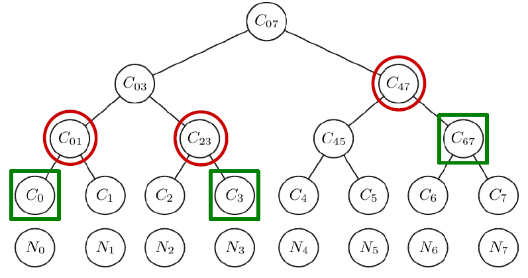
\includegraphics[scale=1.4]{images/3-chiang.png}
% 	\caption{Dynamic Jamming Mitigation --- cover codes (red circle), test code (green square)}%
% 	\label{fig:chiang}
% \end{figure}

\paragraph{Anti-Jamming---Key-Establishment Dependency}
\hl{Above techniques lead to a circular dependency}.
We need techniques without shared secrets!
Idea: \hl{if we cannot coordinate} sender and receiver, then \hl{don't even try}.

\begin{figure}[h]
	\centering
	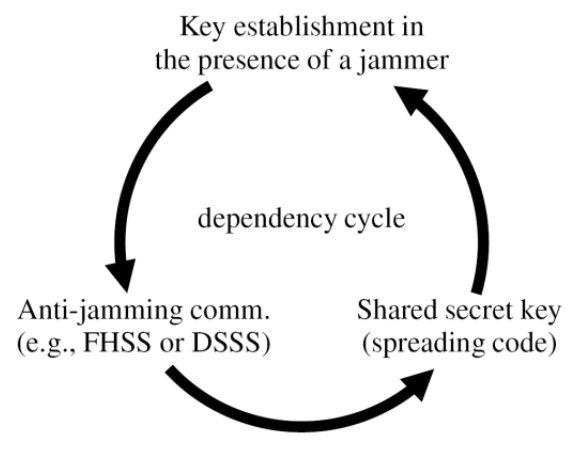
\includegraphics[scale=0.3]{images/3-jamming-key-cycle.png}
	\caption{Circular dependency between anti-jamming and key establishment}%
	\label{fig:jamming-key-cycle}
\end{figure}

In addition, pre-loading shared keys is full of problems:
requires a trusted party, key revocation, new clients joining, etc.

\paragraph{Uncoordinated Frequency Hopping Spread Spectrum UFHSS}
\hl{Neither attacker nor legitimate receivers can predict which channels are used}.
Equivalent to FH in terms of jamming protection (but not in throughput).

Transmitter steps:
\begin{enumerate}
	\item \textbf{Fragment} message
	\item \textbf{Link} fragments (against insertion)
	\item \textbf{Encode packets} (ECC against jamming)
	\item \textbf{Repeated transmission} while hopping on frequencies
\end{enumerate}

Receiver steps: same process but reversed (plus packet ordering).
Hops from one frequency to the other (sequentially is fine), in the hope of receiving a fragment.

\begin{figure}[h]
	\centering
	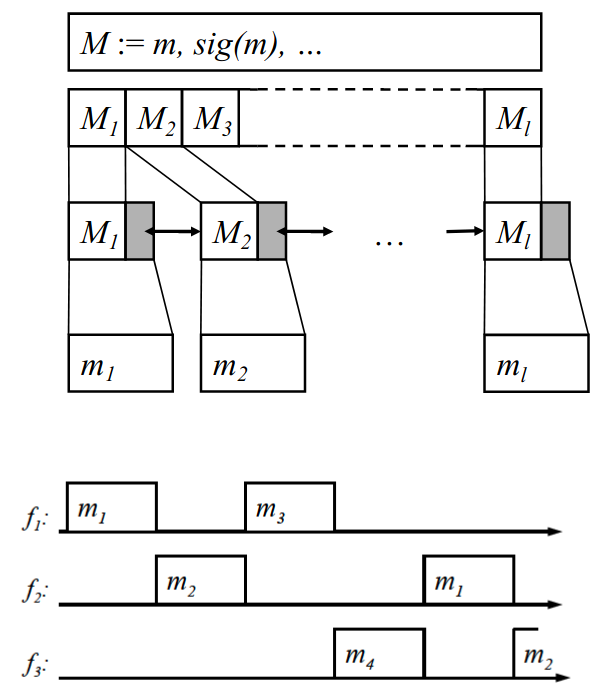
\includegraphics[scale=0.3]{images/3-ufh.png}
	\caption{UFH transmitter steps}%
	\label{fig:ufh}
\end{figure}

\textbf{Issue with fragment linking:} the \hl{signature is only verified at the end} for the entire message.%
\footnote{The signature is based on public-keys and a mutually trusted --- but potentially offline --- certificate authority CA.}
Since there are exponentially many combinations for re-assembly, the attacker can now perform a DoS on a logical (rather than physical) level (pollution attack).
\\
Solution: cryptographic linking of fragments (but without a shared key).
E.g.\ hash linking, one-way accumulators, short signatures.

\textbf{Disadvantages}:
\hl{Throughput up to 1000x less} than Frequency Hopping.
Higher latency (depending on attacker strengths, i.e.\ how high the chances are that the receiver gets a packet).

\begin{figure}[h]
	\centering
	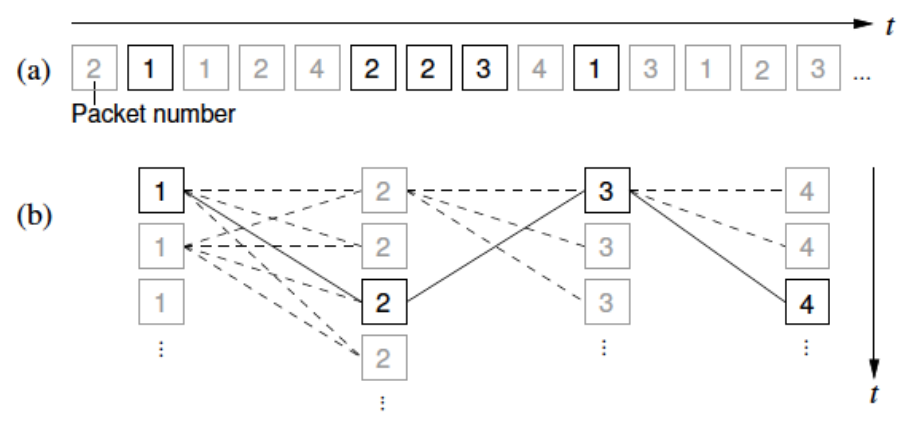
\includegraphics[scale=0.4]{images/3-ufh-fragment-linking.png}
	\caption{UFH fragment linking --- exponentially many candidate messages}%
	\label{fig:ufh-fragment-linking}
\end{figure}

\paragraph{Uncoordinates Direct Sequence Spread Spectrum UDSSS}
Neither attacker nor legitimate receivers can predict which spreading codes are used.
The public code set $C$ is composed of $n$ code sequences, each containing $l$ spreading codes.%
\footnote{This allows a message to be fragmented into $l$ pieces.}
\hl{De-spreading is done by trial-and-error}: it requires the correct code sequence and correct synchronization (which fragment are we at?).
The message is also repeatedly sent because of possible jamming --- possibly in parallel to improve throughput.

\underline{Optimization}: first transmit the message $M$ with a secret spreading code $K$ using DSSS.\@ Then transmit the spreading code $K$ using UDSSS.\@

\underline{Advantage}: quicker decoding, longer messages, flexible security level.


